% Credits are indicated where needed. The general idea is based on a template by Vel (vel@LaTeXTemplates.com) and Frits Wenneker.

\documentclass[11pt, a4paper]{article} % General settings in the beginning (defines the document class of your paper)
% 11pt = is the font size
% A4 is the paper size
% “article” is your document class

%----------------------------------------------------------------------------------------
%	Packages
%----------------------------------------------------------------------------------------

% Necessary
\usepackage[german,english]{babel} % English and German language 
\usepackage{booktabs} % Horizontal rules in tables 
% For generating tables, use “LaTeX” online generator (https://www.tablesgenerator.com)
\usepackage{comment} % Necessary to comment several paragraphs at once
\usepackage[utf8]{inputenc} % Required for international characters
\usepackage[T1]{fontenc} % Required for output font encoding for international characters

% Might be helpful
\usepackage{amsmath,amsfonts,amsthm} % Math packages which might be useful for equations
\usepackage{tikz} % For tikz figures (to draw arrow diagrams, see a guide how to use them)
\usepackage{tikz-cd}
\usetikzlibrary{positioning,arrows} % Adding libraries for arrows
\usetikzlibrary{decorations.pathreplacing} % Adding libraries for decorations and paths
\usepackage{tikzsymbols} % For amazing symbols ;) https://mirror.hmc.edu/ctan/graphics/pgf/contrib/tikzsymbols/tikzsymbols.pdf 
\usepackage{blindtext} % To add some blind text in your paper

\usepackage{graphicx,subfigure}


%---------------------------------------------------------------------------------
% Additional settings
%---------------------------------------------------------------------------------

%---------------------------------------------------------------------------------
% Define your margins
\usepackage{geometry} % Necessary package for defining margins

\geometry{
	top=2cm, % Defines top margin
	bottom=2cm, % Defines bottom margin
	left=2.2cm, % Defines left margin
	right=2.2cm, % Defines right margin
	includehead, % Includes space for a header
	%includefoot, % Includes space for a footer
	%showframe, % Uncomment if you want to show how it looks on the page 
}

\setlength{\parindent}{15pt} % Adjust to set you indent globally 

%---------------------------------------------------------------------------------
% Define your spacing
\usepackage{setspace} % Required for spacing
% Two options:
\linespread{1.5}
%\onehalfspacing % one-half-spacing linespread

%----------------------------------------------------------------------------------------
% Define your fonts
\usepackage[T1]{fontenc} % Output font encoding for international characters
\usepackage[utf8]{inputenc} % Required for inputting international characters

\usepackage{XCharter} % Use the XCharter font


%---------------------------------------------------------------------------------
% Define your headers and footers

\usepackage{fancyhdr} % Package is needed to define header and footer
%\pagestyle{fancy} % Allows you to customize the headers and footers

%\renewcommand{\sectionmark}[1]{\markboth{#1}{}} % Removes the section number from the header when \leftmark is used

% Headers
\lhead{} % Define left header
\chead{\textit{}} % Define center header - e.g. add your paper title
\rhead{} % Define right header

% Footers
\lfoot{} % Define left footer
\cfoot{\footnotesize \thepage} % Define center footer
\rfoot{ } % Define right footer

%---------------------------------------------------------------------------------
%	Add information on bibliography
\usepackage{natbib} % Use natbib for citing
\usepackage{har2nat} % Allows to use harvard package with natbib https://mirror.reismil.ch/CTAN/macros/latex/contrib/har2nat/har2nat.pdf

% For citing with natbib, you may want to use this reference sheet: 
% http://merkel.texture.rocks/Latex/natbib.php

%---------------------------------------------------------------------------------
%	General information
%---------------------------------------------------------------------------------
\title{Spiking Neural Network for Speech Intonation Modeling} % Adds your title
\author{
Lo\"{i}c Jeanningros % Add your first and last name
\\
Idiap Research Institute, Martigny, Switzerland
    %\thanks{} % Adds a footnote to your title
    %\institution{Idiap Research Institute, Martigny, Switzerland} % Adds your institution
  }


\date{\small \today} % Adds the current date to your “cover” page; leave empty if you do not want to add a date


%---------------------------------------------------------------------------------
%	Define what’s in your document
%---------------------------------------------------------------------------------

\begin{document}


% If you want a cover page, uncomment "%---------------------------------------------------------------------------------
% Cover page
%---------------------------------------------------------------------------------

% Here are more templates for other cover pages: https://www.latextemplates.com/cat/title-pages

% This example is based on this cover page example: https://www.latextemplates.com/template/academic-title-page

\begin{titlepage} % Starts new environment where the page number is not displayed and the count starts at 1 for the next page

%------------------------------------------------
%	Institutional information
%------------------------------------------------
	
\begin{minipage}{0.4\textwidth} % Begins new environment (like a text box)
    \begin{flushleft} % Sets environment on the left side of the paper
    \large
    University of XX\\ % Add your institution
    Chair of Political Science IV\\ % Add the chair
    Fall 2018\\ % Add term
    COURSE TITLE\\ % Add course title
    Supervisor: NAME % Add instructor/supervisor name 
    \end{flushleft}
\end{minipage}
	
\vspace*{2in} % Adds some space in-between
	
\center % Centre everything on the page

%------------------------------------------------
%	Main part
%------------------------------------------------
	
{\huge\bfseries TITLE OF YOUR PAPER}\\[0.4cm] % Add your paper title 
{\large\today}\\[0.4cm] % Add date (current day)
FIRSTNAME LASTNAME % Add your name
	
\vfill % Adds additional space

%------------------------------------------------
%	General information about the author
%------------------------------------------------

\vfill % Adds additional space

Your contact info \\ % Add your contact info
Your Program \\ % Add info about your program
Semester you are enrolled \\ % Add info about your semester

\vfill % Adds additional space

%------------------------------------------------
%	Word count
%------------------------------------------------

\vfill % Adds additional space
	
Word count: XXXX % To indicate the word count
% How to check words in a LaTeX document: https://www.overleaf.com/help/85-is-there-a-way-to-run-a-word-count-that-doesnt-include-latex-commands
	

	
\end{titlepage}" and uncomment "\begin{comment}" and "\end{comment}" to comment the following lines
%%---------------------------------------------------------------------------------
% Cover page
%---------------------------------------------------------------------------------

% Here are more templates for other cover pages: https://www.latextemplates.com/cat/title-pages

% This example is based on this cover page example: https://www.latextemplates.com/template/academic-title-page

\begin{titlepage} % Starts new environment where the page number is not displayed and the count starts at 1 for the next page

%------------------------------------------------
%	Institutional information
%------------------------------------------------
	
\begin{minipage}{0.4\textwidth} % Begins new environment (like a text box)
    \begin{flushleft} % Sets environment on the left side of the paper
    \large
    University of XX\\ % Add your institution
    Chair of Political Science IV\\ % Add the chair
    Fall 2018\\ % Add term
    COURSE TITLE\\ % Add course title
    Supervisor: NAME % Add instructor/supervisor name 
    \end{flushleft}
\end{minipage}
	
\vspace*{2in} % Adds some space in-between
	
\center % Centre everything on the page

%------------------------------------------------
%	Main part
%------------------------------------------------
	
{\huge\bfseries TITLE OF YOUR PAPER}\\[0.4cm] % Add your paper title 
{\large\today}\\[0.4cm] % Add date (current day)
FIRSTNAME LASTNAME % Add your name
	
\vfill % Adds additional space

%------------------------------------------------
%	General information about the author
%------------------------------------------------

\vfill % Adds additional space

Your contact info \\ % Add your contact info
Your Program \\ % Add info about your program
Semester you are enrolled \\ % Add info about your semester

\vfill % Adds additional space

%------------------------------------------------
%	Word count
%------------------------------------------------

\vfill % Adds additional space
	
Word count: XXXX % To indicate the word count
% How to check words in a LaTeX document: https://www.overleaf.com/help/85-is-there-a-way-to-run-a-word-count-that-doesnt-include-latex-commands
	

	
\end{titlepage}

%\begin{comment}
\maketitle % Print your title, author name and date; comment if you want a cover page 

%\end{comment}


\setcounter{page}{1} % Sets counter of page to 1



%%%%%%%%%%%%%%%%%%%%%%%%%%%%%%%%%%%%%%%%%%%%%%%%%%%%%%%%%%%%%%%%%%%%%%%%%%%%%%%%
\begin{abstract}
Understanding the mechanisms behind the production of speech intonation requires a physiological model of the pitch production process. Intonation is fully characterized by the fundamental frequency ($f0$) of the speech signal that relies on laryngeal muscles. The Generalized Command-Response (GCR) model that is used approximates muscle dynamics in response to neural spikes. For this reason, a Spiking Neural Network is proposed to learn the sequences of spikes driving muscle responses. It is a spike-based reservoir network inspired from neocortical neural microcircuits called the Liquid State Machine (LSM). It allows to process continuous input streams into a high-dimensional state performing diverse operation and integration of both present and past inputs. Motor commands are extracted from the LSM through Remote Supervison (ReSuMe and SPAN learning rules) in an online manner. Such online computations that transform time-varying input streams into time-varying output streams have never been applied to intonation before. An analysis of the LSM's separation property as well as a comparison of ReSuMe and SPAN algorithm are provided. The model can accurately reproduce single speech utterances. However, the prediction of unseen utterances is not achieved. We hypothesize that the generalization failure is due to both motor commands encoding scheme and bad generalization-capability of the presented LSM.
\end{abstract}


%%%%%%%%%%%%%%%%%%%%%%%%%%%%%%%%%%%%%%%%%%%%%%%%%%%%%%%%%%%%%%%%%%%%%%%%%%%%%%%%
\section{Introduction}
Intonation is a prosodic feature of speech that carries non-linguistic information such as emphasis and emotion. As a distorted pitch can change the meaning of a sentence, or can reveal the speaker's emotional state, a good model of intonation is crucial for speech-to-speech translation systems that intend to transfer para-linguistics between languages.

In previous work with colleagues \cite{honnet2015atom}, a physiologically plausible intonation ($f0$) model based on the Command-Response (CR) model of Fujisaki \cite{fujisaki1998command} has been investigated. Then, a Generalized CR (GCR) \cite{schnell2018neural} that extracts atoms from an intonation contour using a matching pursuit algorithm \cite{mallat1993matching} has been presented. Because GCR atoms approximate muscle responses to incoming neural spikes, we propose to use a Spiking Neural Network (SNN) for learning sequences of spikes that generate intonation contours through muscle responses.

Learning in traditional Artificial Neural Network is usually performed by gradient techniques. However, no explicit evaluation of the gradient in SNNs can be made due to the discontinuous-in-time nature of spikes. Nevertheless, indirect approaches have been attempted :
SpikeProp algorithm \cite{bohte2002error} employed difference between desirable and actual time of output spike as error. A supervised spike-based learning algorithm based on a probabilistic approach \cite{pfister2006optimal} optimizes the likelihood of post-synaptic firing by gradient ascent. Nevertheless, these algorithms do not enable learning patterns composed of more than a single or few spikes, respectively.
Another algorithm \cite{huh2018gradient} allows to learn spike trains, but break the all-or-none nature of synaptic currents.

Error back-propagation seems to be inefficient for learning in SNN. Hence, we turned to an alternative to paradigm based on attractor neural networks, called reservoir computing (RC). RC is attractive for non-experts developers due to the simplicity of the training method, it meets the demands for low training cost and real-time processing of many applications \cite{tanaka2019recent}. The basic idea behind this new trend of understanding training is that, as long as a recurrent neural network possesses certain generic properties, supervised adaptation of all interconnection weights is not necessary. Only training a memory-less supervised readout from it is enough to obtain excellent performance in many tasks \cite{lukovsevivcius2012reservoir}. 

The Liquid State Machine (LSM) \cite{maass2002real} is the first spike-based version of reservoir neural networks. It is a high-dimensional network based on neocortex microcircuits observation. Such network can be seen as a kernel on which input signals are projected. Recurrent connections are not trained, thus LSM's activity is task-independent. 
Under certain conditions, the liquid circuit approximates the computation of any linear and nonlinear mathematical operation and also provides all needed temporal integration of information \cite{maass2011liquid}. Since the liquid state has only one attractor: the resting state, inputs can be seen as perturbations liquid state. Thus, readout neurons can learn to extract in real-time from the current perturbed liquid state about current and past inputs. The LSM is a model for real-time computations on continuous streams of data such as spike trains \cite{maass2011liquid}, hence it is appropriate for the intonation production task.

Reservoir computing has recently shown promising performance in various speech processing tasks \cite{triefenbach2014large, triefenbach2010phoneme, ikeda2018short, zhao2018nonlinear}, in particular LSM with a spike-based learning algorithm for speech recognition \cite{zhang2015digital}. However, as far as we know, it has never been applied to speech intonation modelling, and speech synthesis in general. The closest study seems to be an FORCE-trained spike-based reservoir network \cite{nicola2016supervised} that successfully reproduces songbird singing.

Readout neurons learn to extract motor commands from neural circuit information through the plasticity of connections from the reservoir. A couple of Remote Supervision learning rules allow online local synaptic adaptation: SPAN \cite{mohemmed2012span, mohemmed2013training}, that has been adapted in previous work \cite{schnell2018neural} and ReSuMe \cite{ponulak2006supervised, ponulak2010supervised} that has proven itself adequate for learning motor commands. Indeed, SNN trained with ReSuMe become efficient neurocontrollers for movement generation and control due to the ability of the method to operate online and due to its fast convergence \cite{ponulak2010supervised}.

We suppose that readout neurons trained through Remote Supervision can learn to extract the motor commands that generate intonation contours from an LSM receiving phoneme input features. In the following sections, an analysis of the LSM's separation property in response to specific phoneme input features is presented. The learning capabilities of SPAN and ReSuMe are compared and tested on speech intonation modelling. Finally, potential improvements of the model are discussed.


\section{Separation Property}
The first component of a LSM $M$ is an operator or filter $L^M$, called liquid filter or liquid circuit. The liquid state $x^M(t)$ is simply the current output of the liquid filter $L^M$ that maps input functions $u(\cdot)$ onto functions $x^M(t)$ \cite{maass2002real}: \begin{equation}
x^M(t) = (L^M u)(t)
\end{equation}
The liquid state $x^M(t)$ is defined as the vector of output values at time $t$ of linear filters with exponential decay ($\tau_m = 30$ ms) applied to the spike trains emitted by the liquid neurons. It represents all information that a readout neuron could extract at time $t$ from the circuit. The input state can be defined similarly.

The Separation Property (SP) addresses the amount of separation between the trajectories of internal states of the system that are caused by two different input streams. SP is evaluated by injecting pairs of input spike trains $u(\cdot)$ and $v(\cdot)$ and recording resulting trajectories $x_u^M(t)$ and $x_v^M(t)$. 

The distance $d(u,v)$ between two input states is defined as the Euclidean norm of their difference averaged over time and neurons. The state distance $D_{u,v}(t) = \parallel x_u^M(t) - x_v^M(t)\parallel$ is the Euclidean norm of the liquid state difference averaged over neurons.

In order to evaluate LSM's SP, 599 feature combinations that are observable in data are selected as input samples. The LSM is initialized once to its initial state, it is run during 800 ms with unvoiced state feature active. The selected input sample is active in the interval from 300 to 600 ms. The network is restored to its initial state and the simulation is repeated for all input samples.

Pairs of input samples are selected such that their input distance is precisely $d(u,v) =$ 1.21, 2.1, 3.2 or 4.3. 406 pairs are randomly chosen for each input distance and the corresponding liquid state distances are measured. The simulations are repeated three times with the same network structure, but different initial values of the liquid neurons membrane potential, such that the state distance for $d(u,v) = 0$ can also be measured. This experiment is repeated three times with different generated networks. A linear regression allows to extract the slop $\alpha$ and the residuals $r$ of the relation between state and input distances as well as the standard deviation $\sigma$, all of them averaged across time in the interval [300 ms, 700 ms] and experiment repetitions.

SP is often used to optimize neuronal model \cite{hourdakis2013use, wojcik2007liquid, grzyb2009model, wojcik2012electrical}, liquid architecture \cite{hourdakis2013use}, liquid connectivity density ($\lambda$) \cite{hourdakis2013use, grzyb2009model, maass2002real} or synaptic parameters \cite{pipaextended}. SP has even been observed from \textit{in vitro} cultured cortical networks \cite{dockendorf2009liquid}

Whereas, in these studies, inputs are often modeled as spike trains generated from a Poisson distribution of frequency in the order of 20 Hz (max. 50 Hz) from a limited number of neurons (a few up to 81), our phoneme inputs are composed of 374 input channels (max. 15 simultaneously active) regularly spiking at 200 Hz. Due to the specificity of our inputs, SP analysis is performed in order to optimize parameters of connections from inputs to LSM (probability of connection $p_i$ and $p_{vuv}$ and synaptic weights $w_i = w_{vuv}$) and intra-reservoir connections (density of connections $\lambda$). Simulations have been performed with a LSM of dimensions $8 \times 8 \times 16$.

As the probability of connection $p_i$ increases, $\alpha$, $r$ and $\sigma$ increase (not shown). The value $p_i = 0.015$ is chosen such that $r$ and $\sigma$ remain acceptable. When $p_{vuv}$ increases $\alpha$ decreases, but $r$ and $\sigma$ are large for small values of $p_{vuv}$. The rise of liquid state activity for the very first input stimulation is a typical observation in LSM studies. It is certainly due to the short-term memory of liquid synapses that release a larger amount of current when the presynaptic neuron did not fire recently. VUV state inputs allow to start the network activity before presenting input samples and to constantly maintain a minimal network activity during the simulations. $p_{vuv} = 0.1$ is chosen in that purpose. Difference between SP experiments where LSM is stimulated by VUV state inputs or not can be observed on Figure \ref{SPvuv}. The liquid state shows a chaotic behavior when the stimulation starts, at $t=0$ ms if VUV state inputs are connected and at $t=300$ ms if they are not, distorting the liquid response to phoneme inputs in the latter case.

\begin{figure}
\center
\subfigure{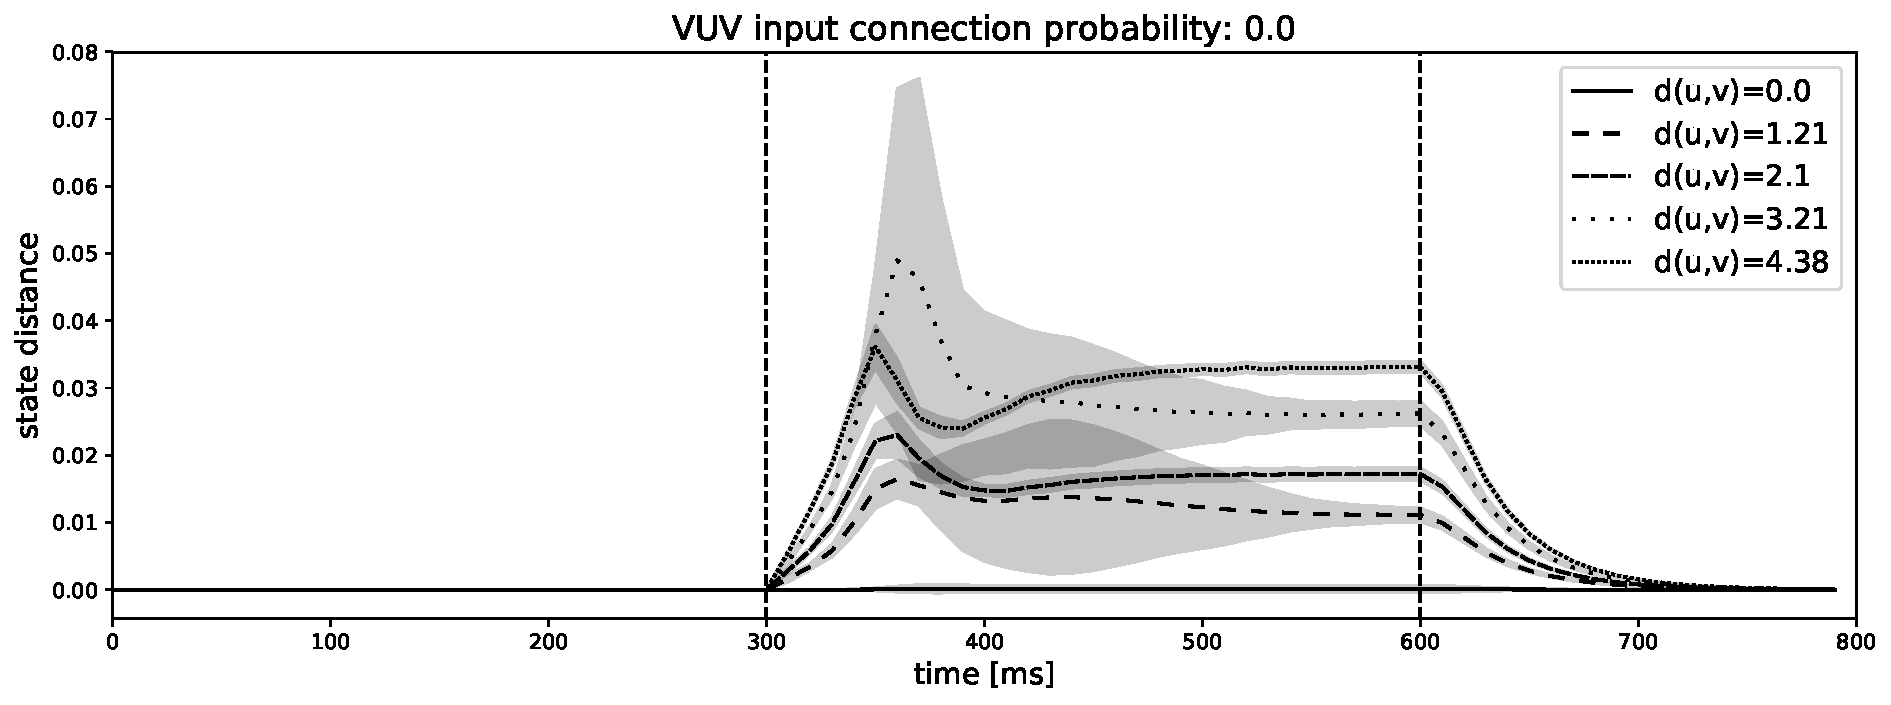
\includegraphics[scale=.47]{figures/SP_Pvuv_00.pdf}}
\subfigure{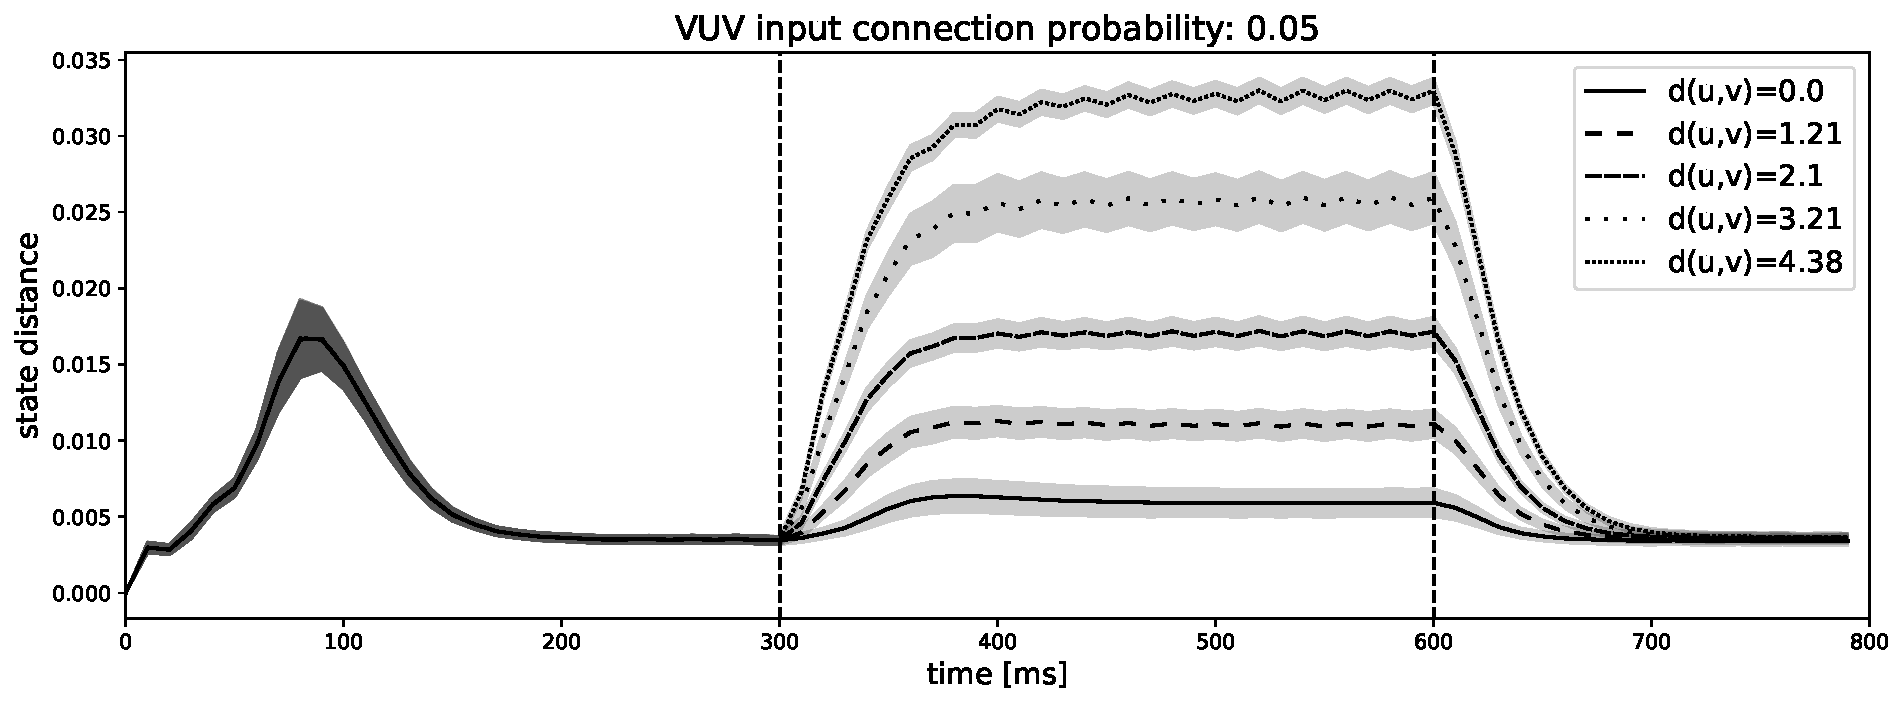
\includegraphics[scale=.47]{figures/SP_Pvuv_005.pdf}}
\caption{Liquid state distance $D_{u,v}$ as a function of time for different input distances $d(u,v)$. Liquid state distances are not proportional to input distances when VUV state inputs are not connected (top). Good proportionality is achieved with VUV state inputs connected (bottom) due to an earlier chaotic activation of the LSM (0-200 ms)}
\label{SPvuv}
\end{figure}

As the synaptic weights $w_i$ increase, $\alpha$ increases and below $w_i = 60$ nA both $r$ and $\sigma$ are reasonable. However, following experiments show that it is more difficult to extract information from the liquid network stimulated with such strength, then $w_i = 5$ nA is chosen. It points out that the Euclidean distance or the SP itself could be insufficient measures. Some other studies perform entropy measures or auto-correlation functions. Also, the generalization property as to be considered in addition to SP for good learning performances (see Discussion). 

The effect of $\lambda$ on the SP is very interesting (Figure \ref{SPlambda}). $\lambda$ has very little effect on $\alpha$, but both $r$ and $\sigma$ show a peak around $\lambda = 1.7$. After the peak ($\lambda > 1.9$), their values remain superior to what they were before the peak ($\lambda < 1.5$). This could be the transition from a non-chaotic regime to a chaotic regime. However no measure discriminating between non-chaotic and chaotic regimes is performed to confirm such assumption. The value $\lambda = 1.25$ is chosen because when a system parameter variation causes a transition between non-chaotic and chaotic regimes, it is often recommended that the parameter is set close to the transition point \cite{bertschinger2004real, legenstein2007edge}.

\begin{figure}
\centering
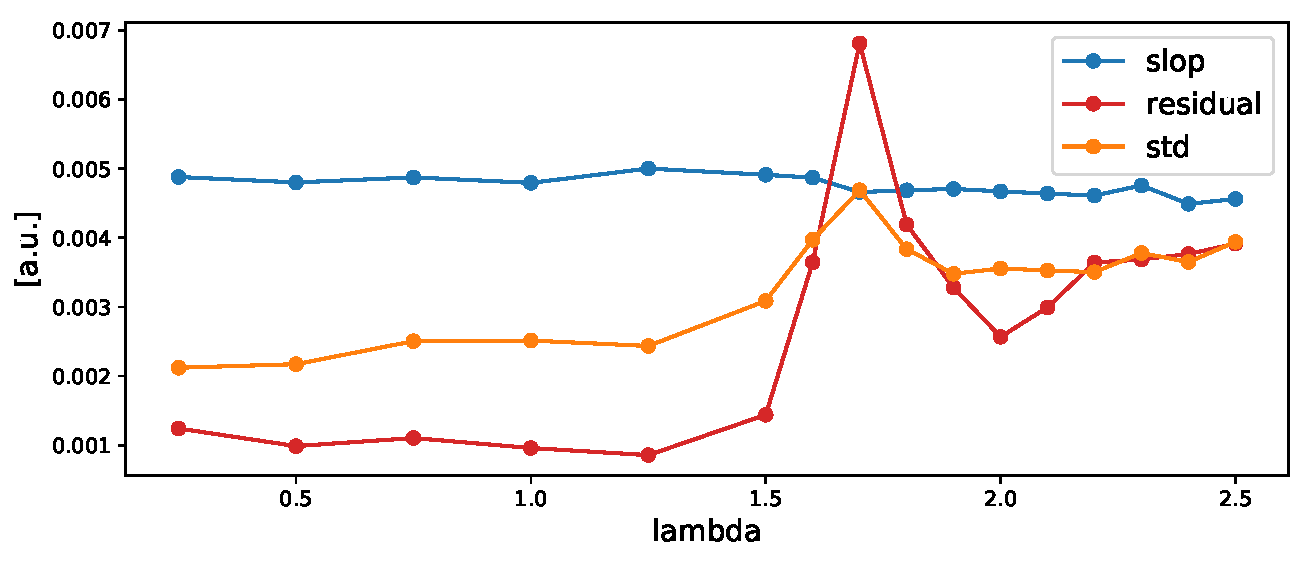
\includegraphics[scale=.7]{figures/SP_lambda.pdf}
\caption{Slope $\alpha$ and residuals $r$ of the linear regression between liquid state distances $D_{u,v}$ and input distances $d(u,v)$, as well as standard deviation $\sigma$ averaged over the time interval [300 700] ms of SP experiment depending on the value of the LSM's density of connections $\lambda$.}
\label{SPlambda}
\end{figure}

\section{Approximation property}

The second component of an LSM $M$ is a memoryless readout map $f^M$ that transforms, at every time $t$, the current liquid state $x^M(t)$ into the output $y(t)$ \cite{maass2002real}: \begin{equation}
y(t) = f^M(x^M(t))
\end{equation}

The set of connections from the LSM network to readout neurons constitute the readout map. These connections are the only ones to be plastic, i.e. trained to reproduce sequences of spikes that generate intonation contours. Two similar learning rules, both derived from Windrow-Hoff rule, are investigated: ReSuMe \cite{ponulak2006supervised, ponulak2010supervised} and SPAN \cite{mohemmed2012span, mohemmed2013training}. Both learning rules belong to Remote Supervision, meaning that an instructive signal (the teacher) induces synaptic weight adaptation without contributing to the postsynaptic neuron dynamics. They are efficient supervised algorithm enabling readout neurons to reproduce the target sequences of spikes with high-precision. They are two main difference between SPAN and ReSuMe. The first one is that: while presynaptic spike trains are filtered by a kernel in both algorithms, ReSuMe uses precise spike times of postsynaptic and teacher neurons whereas SPAN also kernelizes postsynaptic and teacher spike trains. The second difference is the shape of kernels used to filter spike trains: ReSuMe applies an exponential kernel and SPAN an $\alpha$ kernel function. It has been shown that $\alpha$ kernel  function achieves better results than the exponential kernel function. However, online implementation of $\alpha$ kernels implies resolving a second-order differential equation, while a a first-order one describes exponential kernels dynamics. Taking in account that postsynaptic and teacher spike trains have to be kernelized in addition, it leads to a significantly higher computational cost for learning with SPAN.

An other difference that ensued from filtered postsynaptic and teacher spike trains is that a presynaptic spike occuring after both postsynaptic and teacher spikes induce a weight change whereas this presynaptic spike does not contribute to the firing of the postsynaptic neuron at the precise teacher spike time. This allows some flexibility that could be beneficial for generalization, but it violates Hebb's principle \cite{hebb1949organization}. Weight updates of both learning rules are plotted as a function of the presynaptic spike time in Figure \ref{dw}.

\begin{figure}
\centering
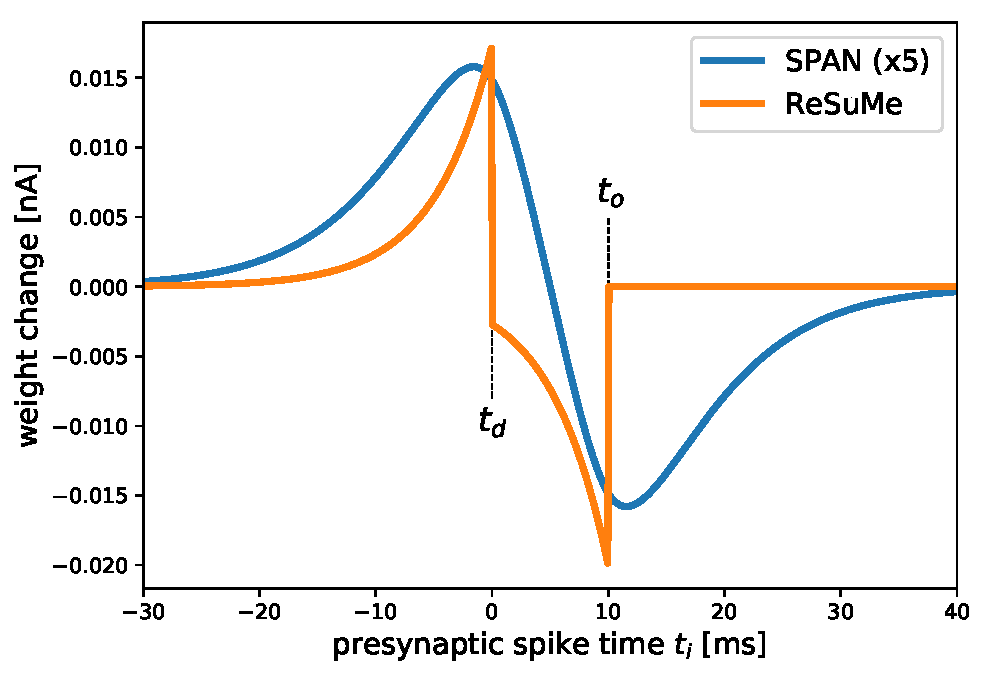
\includegraphics[scale=.7]{figures/weight_update.pdf}
\caption{Weight update as a function of the presynaptic spike time for SPAN and ReSuMe learning rules. Postsynaptic spike time is $t_o = 10$ ms and teacher spike time is $t_d = 0$ ms}
\label{dw}
\end{figure}

Naively, the expected advantage of using SPAN learning rule was that $\alpha$-kernel shape is identical to muscle responses triggered by readout neurons. Thus, the time constant of SPAN kernels could have been in the order of muscle's time constant. However, long kernel shapes cannot lead to good learning performances with an online implementation of SPAN. This is due to the summation of presynaptic kernels since multiple presynaptic spikes occur within the kernel length. Better performance is obtained with short kernel's time constant ($\tau = 15$ ms is chosen), in the order of membrane potential dynamics rather than muscle dynamics, as presented in Figure \ref{SPANtheta}. Thus, SPAN learning behavior becomes very similar to ReSuMe with a significantly higher computational cost.

\begin{figure}
\centering
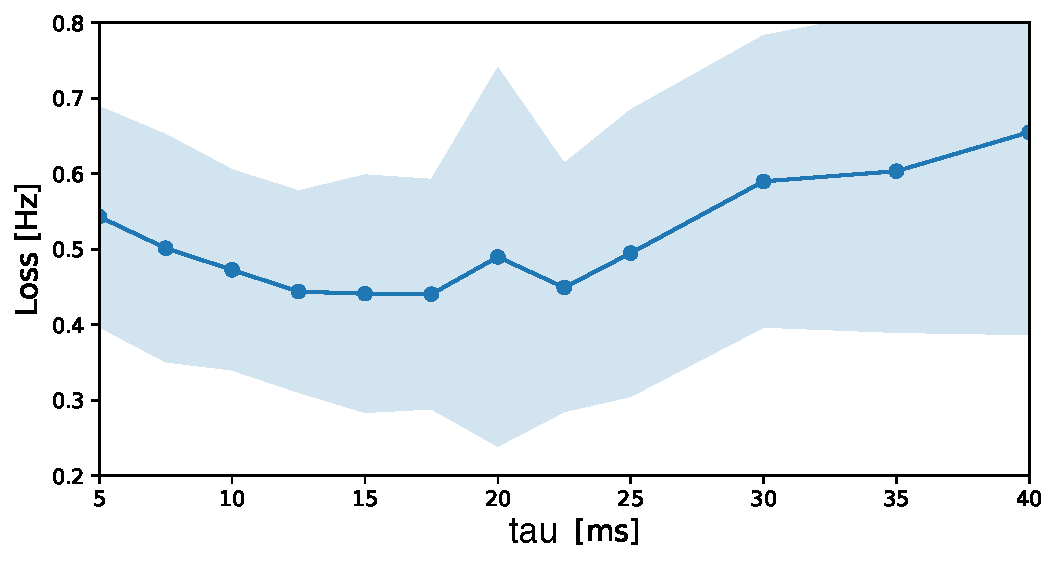
\includegraphics[scale=.7]{figures/SPANtheta.pdf}
\caption{RMS loss between teacher and output LF0 curves as a function of SPAN time constant $\tau$}
\label{SPANtheta}
\end{figure}

\begin{figure}
\center
\subfigure{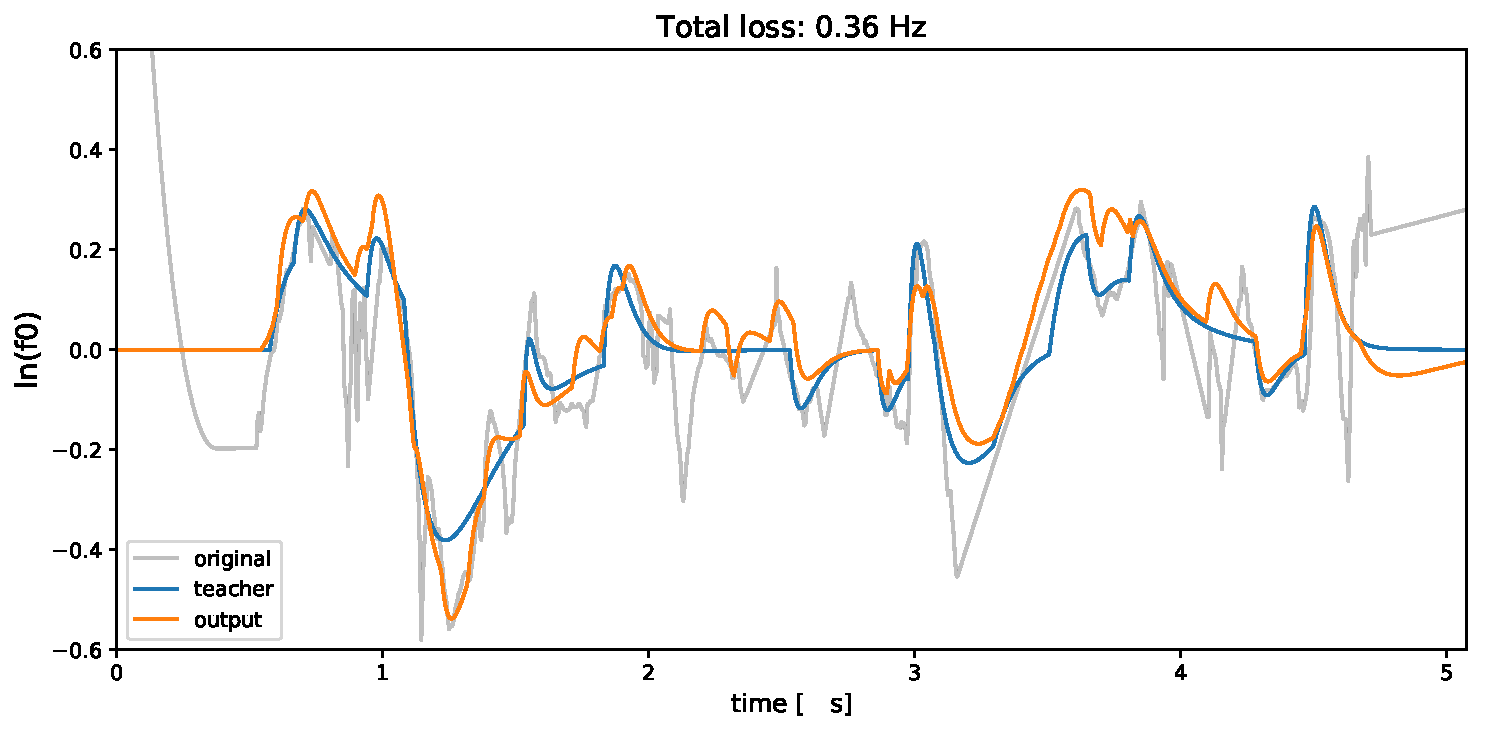
\includegraphics[scale=.42]{figures/job44_SPAN.pdf}}
\subfigure{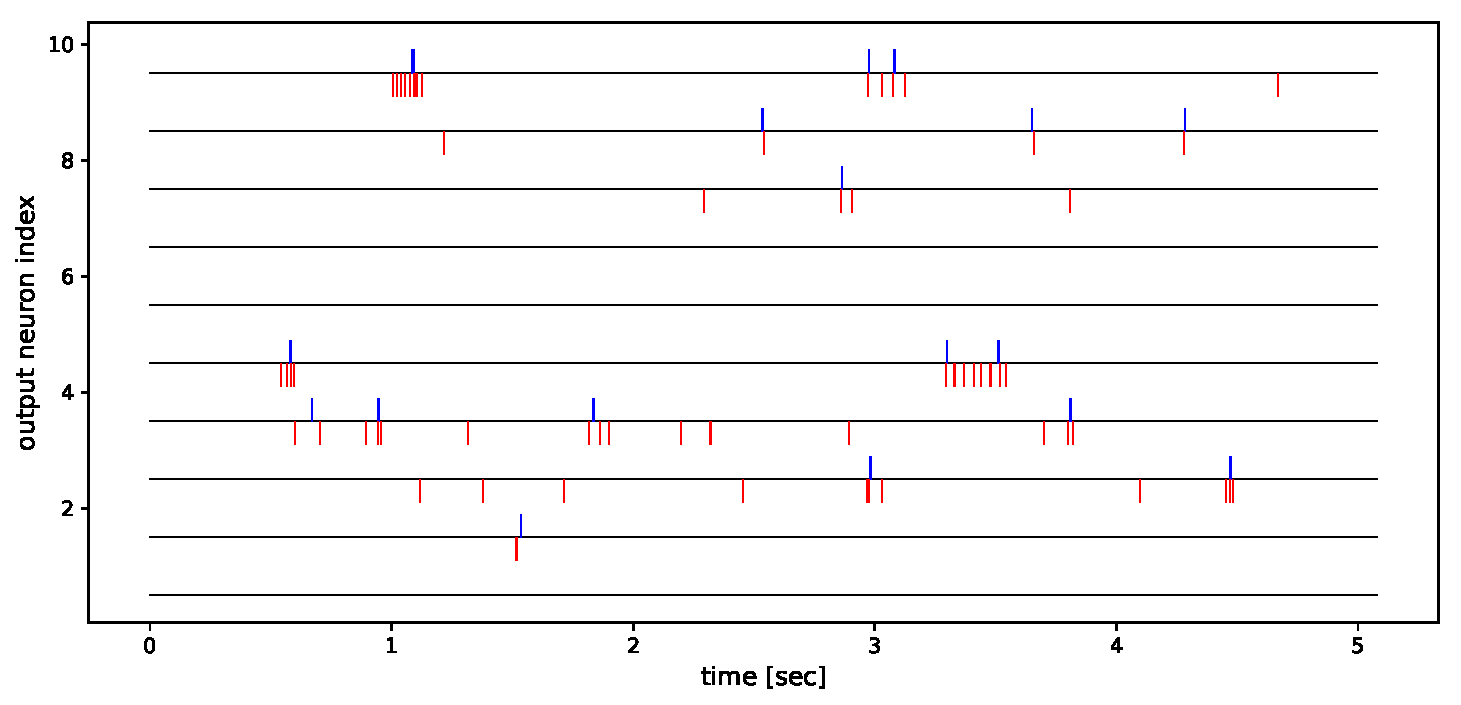
\includegraphics[scale=.42]{figures/job44_roger_5382_spikes.pdf}}
\caption{Top: Reproduction of LF0 teacher signal (after subtraction of a phrase component) with ReSuMe learning rule. Bottom: Reproduction of teacher spike trains (motor commands). Output spikes are red and teacher spikes blue for ten muscles}
\label{singleSampleR}
\end{figure}

\begin{figure}
\center
\subfigure{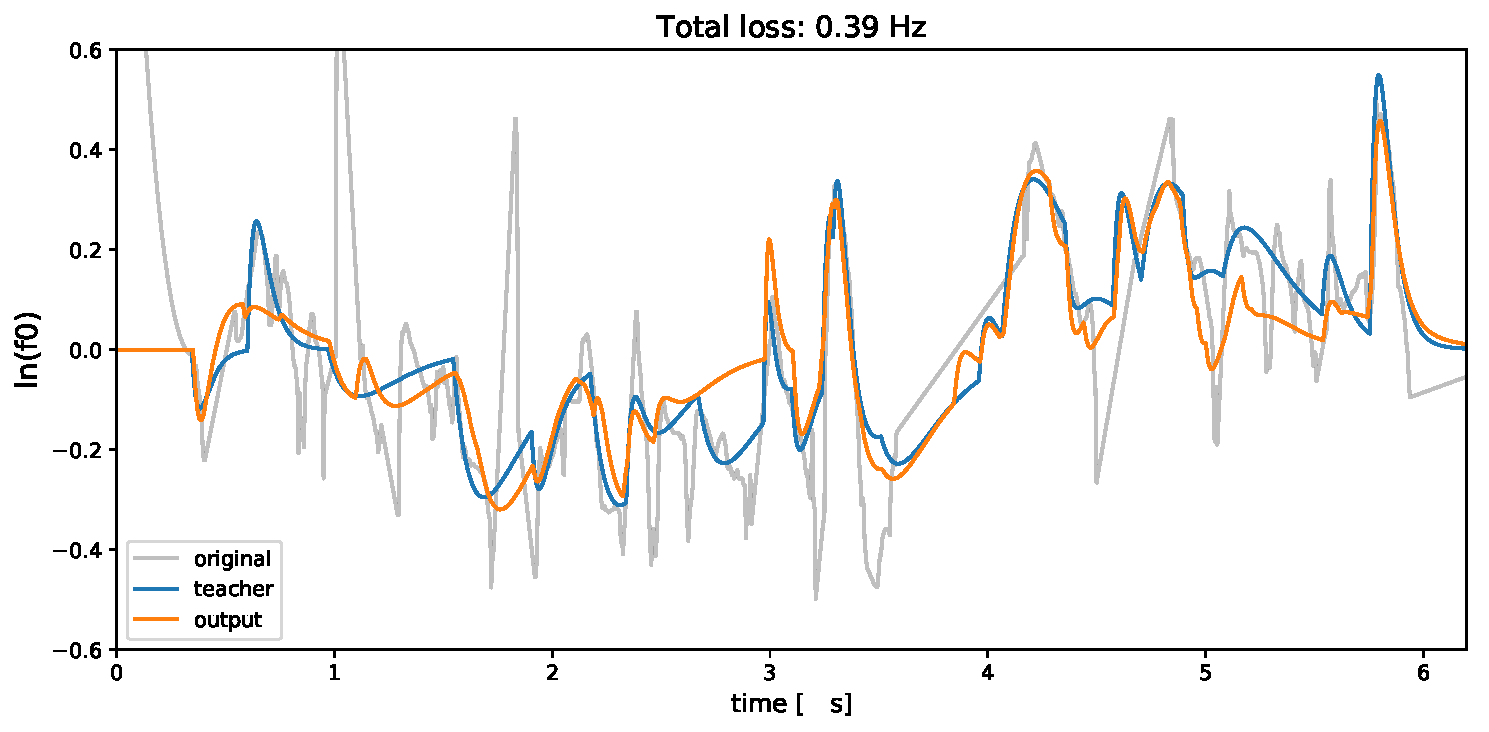
\includegraphics[scale=.42]{figures/job23_ReSuMe.pdf}}
\subfigure{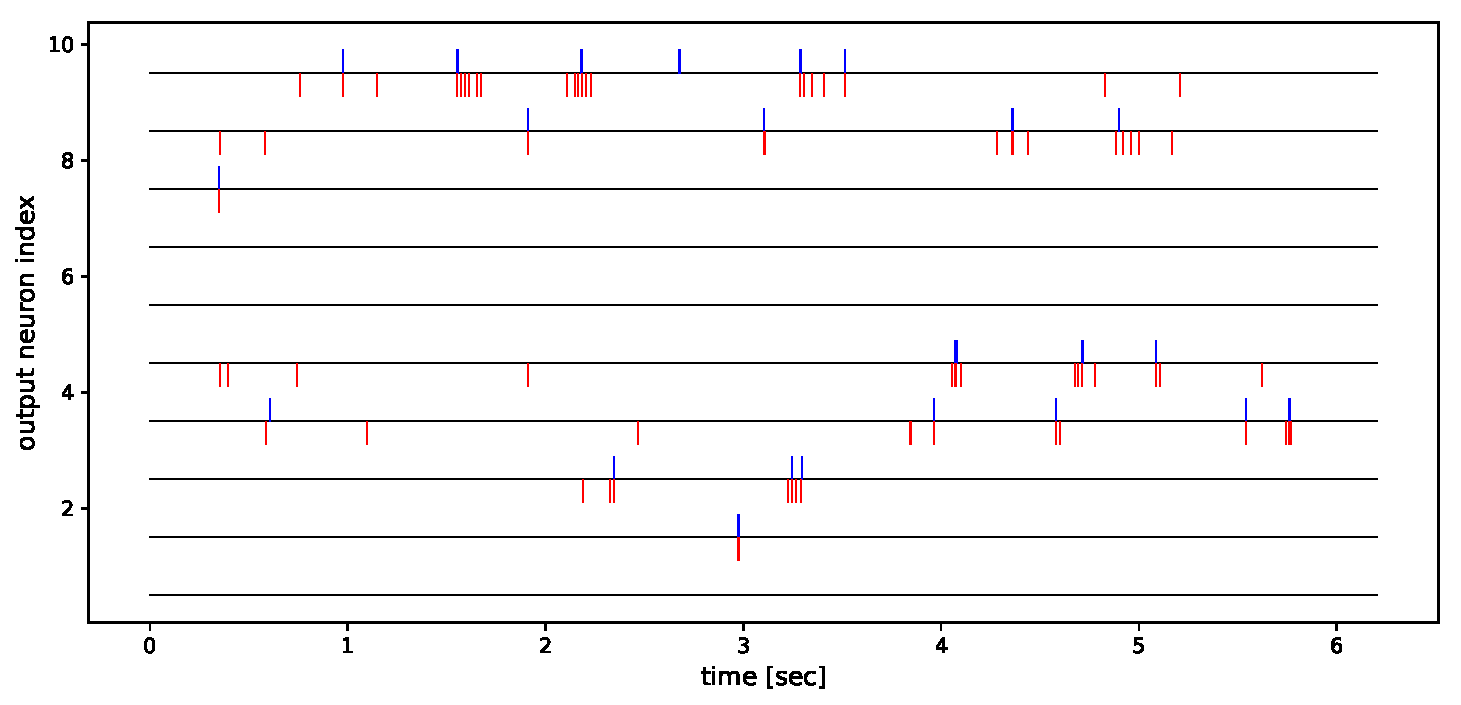
\includegraphics[scale=.42]{figures/job23_roger_5421_spikes.pdf}}
\caption{Same than Figure \ref{singleSampleR} on a different sample with SPAN learning rule}
\label{singleSampleS}
\end{figure}

ReSuMe (Figure \ref{singleSampleR}) and SPAN (Figure \ref{singleSampleS}) are both accurately reproducing a single sample after learning (ReSuMe performs slightly better than SPAN). However, none of them converges to the exact solution. As a consequence, synaptic weights magnitude continues to increase after the best performance is reached. From these results, it appears that the learning task is very complex to solve, otherwise the optimal solution would have been reached easily. It has been supposed that the difficulty could come from the fact that readout neurons have to be repeated several times in order to approximate the amplitude of motor commands. Then, multiple readout neurons have been trained to trigger the dynamic of the same muscle, such that a motor command represents maximum two spikes per readout neuron. This alternative encoding scheme did not lead to any performance improvement.

\begin{figure}
\centering
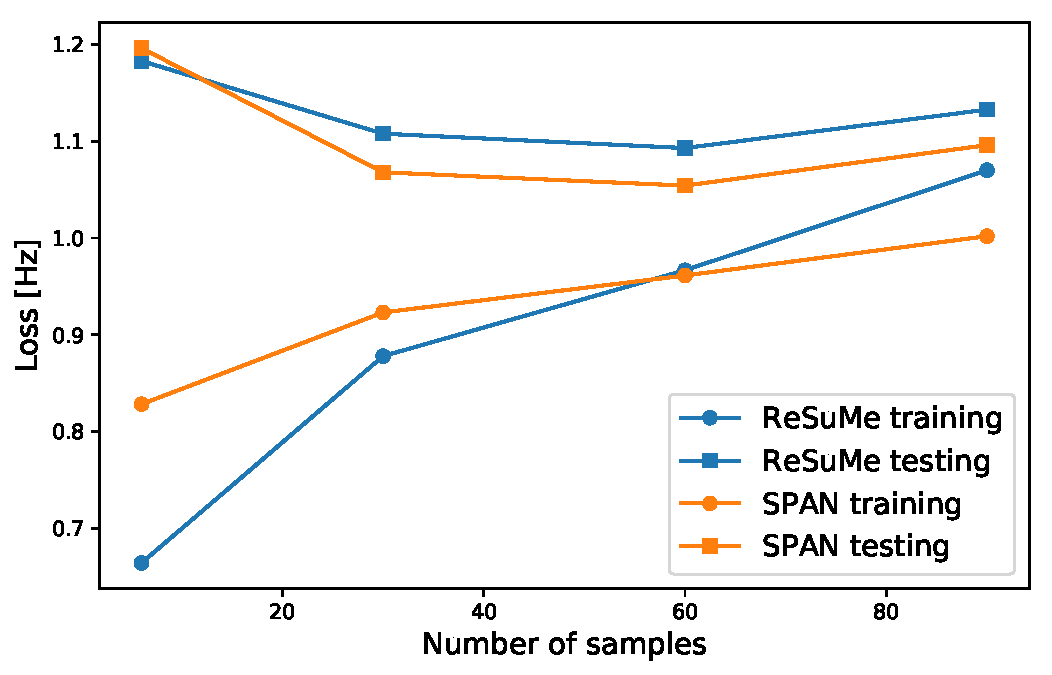
\includegraphics[scale=.7]{figures/CV.pdf}
\caption{Prediction performance of ReSuMe and SPAN learning rules as a function of the total number of samples used for the 6-fold cross-validation}
\label{multipleSample}
\end{figure}

Figure \ref{multipleSample} shows that the model does not generalize, i.e. training on multiple samples does not allow to predict unseen samples. The training error increases significantly with the number of learned samples, confirming that the learning task is very complex. The testing error remains large independently of the number of learned samples. This generalization failure is discussed in the following section. It has been supposed that the size of the neural network could improve performance, it effectively slightly decreases the training error, but no significant improvement for generalization.


\section{Discussion}

%\subsection{Biological relevance}
%Brain regions
%Learning rules

%\subsection{Future directions}

The Liquid State Machine allows to process continuous streams of multiple input. Readout neurons can learn to extract in an online manner from the current state of such recurrent circuit information about current and past inputs. Such online processing and extraction of information has never been used in Text-To-Speech before. This spiking reservoir network model can learn to reproduce intonation contours of utterances with high accuracy. However, our model is not capable of generalization, meaning that the intonation's prediction of unseen utterances has not been achieved.

It has been demonstrated that spiking neurons trained with ReSuMe are able to transform inputs to the desired output spike trains for the patterns not used during the training \cite{ponulak2006generalization}. In that sense, neurons trained with ReSuMe demonstrate the generalization property, then the learning rule is not responsible for the generalization failure. The inability of readout neurons to extract motor commands from the liquid state means that either the liquid state does not provide underlying information needed for generalization, or desired motor commands (i.e. teacher spike trains) does not represent a generalizable signal of intonation contours, or both.

\paragraph{Motor commands}
Motor commands, which are the spike trains triggering muscle responses could be unsuitable for generalization. Indeed, output spike trains are encoded such that several spikes (max. 16) confined in a very short time window (one spike every 2.2 ms) trigger a long muscle response (tens to hundreds of milliseconds). Then, output spike trains may be too sparse to be a generalizable signal. One solution would be to encode motor commands with a larger number of spikes distributed on a longer time period. In this way, output neurons would extract motor commands from periodic/regular activity of the liquid state rather than information available at a specific time. The periodic nature of the liquid state in response to phoneme inputs promotes such an alternative output encoding scheme. In addition, it makes sens that generalization emerges from features of the liquid state that are periodic/permanent rather than spontaneous. This alternative encoding scheme corresponds to the approximation of a continuous muscle stimulation by a repetition of spikes on a given time period. It is supported by the original version of the Command-Response model \cite{ohno1998effects} where accent commands are continuous step functions of time.

This alternative encoding scheme raises a particular problem: the pursuit algorithm used for extracting output spike times from intonation contours cannot generate such repetitions of spikes. However, the superposition of gamma kernels of order two from repeated spikes can probably approximate a gamma kernel of higher order. It would give the opportunity to extract muscle responses as higher-order gamma kernels with a matching pursuit algorithm and encoding output spike trains by the related superposition of order-2 gamma kernels for the learning task. Such relations between gamma-kernels orders should be investigated first.

%In addition, it is probable that output spike times extracted by a matching pursuit algorithm do not approximate sufficiently accurately the ground truth for generalization. Supervised learning rules require access to an exact copy of the target response, in our case output spike trains extracted with the pursuit algorithm. However, a novel learning algorithm for reservoir computing models the interaction between reinforcement learning in the basal ganglia and unsupervised learning in cortical pathways \cite{pyle2018model}. Such learning alternative would enable to learn motor commands (output spike trains) by directly using the difference between the original and the generated lf0 signals as a reward rather than falling back on matching pursuit algorithm.

\paragraph{LSM generalization property}

Although separation property is useful for characterizing the reservoir's network ability to separate different inputs, enhancing that property only allows to decrease the training error, in other words, to reproduce samples used for training. It would have been judicious to measure the reservoir's ability to predict unseen samples, named the generalization property. A study on prediction of computational performance for spike-based reservoir networks \cite{legenstein2007edge} not only measure the generalization-capability of the LSM, but present a more accurate measure of the separation property. The generalization-capability can be quantified in terms of the VC-dimension \cite{vapnikn}. It is demonstrated and explained why computational performances are maximal  at the "edge of chaos", by measuring both kernel-quality (SP) and generalization-capability.

\paragraph{Feedback}

Recent studies often resolve learning tasks with reservoir networks working in a different regime \cite{jaeger2004harnessing, sussillo2009generating, nicola2016supervised}. They generate reservoir networks that show spontaneous chaotic activity in absence of input stimulation. It has been shown in the original proposition of FORCE learning \cite{sussillo2009generating}, that there are significant advantages using a network that exhibits chaotic activity prior to training: smaller number of required training periods, better performance, and smaller magnitude of the readout weight vector. However, chaotic activity during training must be avoided. The critical element for suppressing chaos is a feedback loop that carries the output back into the reservoir network. In the presence of feedback loop, output errors must be small enough to be fed back without introducing significant delayed effects that disrupt learning. To this end, synaptic modifications must be strong and rapid during the initial phases of training. As a result, the goal of training is not to significantly reduce error, but rather reducing the amount of modification needed to keep the errors small. ReSuMe appears ideal for such training paradigm due to its fast convergence. In particular, it appeared that the parameter $a_d$ enables rapid synaptic changes allowing for low-error training. That parameter could be reduced as training progresses.

In a first attempt on computing with feedback, it would be pertinent to start with a rate-based reservoir network model, the Echo-State Network (ESN). This would simplify network dynamics while a spike-based neuron model can still be used for readout neurons. Then, a study of a FORCE trained reservoir \cite{nicola2016supervised} provides a deep analysis on spike-based reservoir networks with feedback.

The fact that feedback would help for better performance and in particular generalization is based on the following intuition: it is very difficult for a human to learn how to speak without hearing its own voice. However, cited studies which used feedback with a reservoir network have reproduced complex signals, but none of them performed a prediction task.

\section{Methods \label{methods}}
\subsection{Inputs}
Input data are from the speech database released for the Blizzard Challenge \cite{karaiskos2008blizzard} on a subset (carroll, arctic, theherald 1,2,3) of the native English Voice A (Roger) of about $17.5$ minutes (169 utterances). 374 binary features are extracted from it (see Experimental Setup in previous work \cite{schnell2018neural}) which represent past, current and following phonemes. These features are converted into spike trains by setting a spike generator for each feature. A spike is emitted at every frame (5 ms) when the corresponding feature is equal to one.
A spike generator has a probability $p_i$ to be connected with each neuron of the LSM and $w_i = 5$ nA is the amount of current transmitted by a spike to the postsynaptic neuron. 

The voiced/unvoiced flag is also taken as an input signal represented by a couple of spike generators that emit spikes regularly at $200$ Hz either during voiced or unvoiced periods. $p_{vuv}$ is the probability of connection to liquid neurons and $w_{vuv} = 5$ nA their synaptic weights.

The synaptic delays of inputs are randomly generated from a uniform distribution in the interval [0 ms, 5 ms].

\subsection{Liquid State Machine}

The LSM's neural components and topology are identical to its original description \cite{maass2002real} except for the background current $I_b$. The network is a column in space of $N = 1024$ Integrate-and-Fire neurons, 20\% of which is chosen to be inhibitory. Some parameters depends on whether the neuron is excitatory (E) or inhibitory (I).
\paragraph{Neuronal parameters}
The membrane potential dynamic is driven by the equation :
\begin{equation}
\tau_m \dot{v}(t) = -(v(t)-v_{rest}) + R_m (I_e(t) + I_i(t) + I_b)
\label{IaF}
\end{equation}
where the membrane time constant $\tau_m = 30$ ms, the resting potential $v_{rest} = 0$ mV, the membrane resistance $R_m = 1$ M$\Omega$ and the background current $I_b$ is randomly chosen from uniform distribution between 13.5 and 14.5 nA. The postsynaptic currents coming from excitatory $I_e(t)$  and inhibitory $I_i(t)$ presynaptic neurons are modeled as exponential decay with respect to time constant $\tau_e = 3$ ms and $\tau_i = 6$ ms:
\begin{equation}
\tau_{e,i} \dot{I}_{e,i}(t) = -I_{e,i}(t)
\end{equation}
When the membrane potential crosses the threshold potential $v_{th} = 15$ mV, the neuron emits a spike. Its membrane potential is reset to a reset potential $v_{reset} = 13.5$ mV and is insensitive to incoming currents ($v = v_{reset}$) during a refractory period $t_{ref}$ of 3 ms (E) or 2 ms (I).

\paragraph{Connectivity structure}
The probability of connection from neuron $a$ to neuron $b$ is defined as $C e^{-(D(a,b)/\lambda)^2}$, where $\lambda$ is a parameter that controls both the average number of connections and the average distance between neurons that are synaptically connected. $N$ neurons are located on the integer points of a $8 \times 8 \times 16$ column in space, where $D(a,b)$ is the Euclidean distance between neurons $a$ and $b$. The value of $C$ is 0.3 (EE), 0.2 (EI), 0.4 (IE), 0.1 (II).

\paragraph{Synaptic connections} The synaptic dynamics are driven by Tsodyks model \cite{maass2002synapses} (which corrects a small error in \cite{markram1998differential}). The dynamics of the usage of releasable neurotransmitter per single action potential $u$ and the fraction of synaptic neurotransmitter resources available $x$ have been adapted from discrete time formulation to differential formulation as it follows : \begin{equation}
F \dot{u} = -u \quad \textnormal{and} \quad D \dot{x} = 1-x
\end{equation}
with following actions triggered by presynaptic spikes: \begin{equation}
r = u \cdot x, \quad x \mathrel{-}= r \quad \textnormal{and} \quad u \mathrel{+}= U(1-u)
\end{equation}
The synaptic parameters $U$ (use), $D$ (time constant for depression) and $F$ (time constant for facilitation) are randomly chosen from Gaussian distribution. The mean values of these three parameters (with $D$ and $F$ expressed in second) are .5, 1.1, .05 (EE), .05, .125, 1.2 (EI), .25, .7, .02 (IE), .32, .144 and .06 (II). The standard deviation of each parameter is 50\% of its mean value (with negative values replaced by values chosen from an appropriate uniform distribution). The mean of the scaling parameter A (in nA) is 30 (EE), 60 (EI), -19 (IE) and -19 (II). The standard deviation of the paramater A is 100\% of its mean and is drawn from a Gamma distribution. The transmission delays between liquid neurons are 1.5 ms (EE) and 0.8 ms for other connections. For each simulation, the membrane voltage at $t=0$ is randomly chosen from a uniform distribution from interval [13.5 mV, 15 mV].

\subsection{Learning rules}
Synaptic weights of both learning rules are initialized from a Gaussian distribution of mean 0 nA and width 0.01 nA and learning sessions are always 100 repetitions of the training set.

\paragraph{ReSuMe}
ReSuMe learning rule is derived from Windrow-Hoff algorithm proposed for rate based neuron models. It is adapted to spiking neuron model using the interaction between two spike-timing dependent plasticity processes \cite{ponulak2010supervised}. The final formulation describes the adaptation of synaptic weight between presynaptic neuron $i$ and postsynaptic neuron $o$ in real-time : \begin{equation}
\dot{w}_{oi}(t) = \left[ S_d(t) - S_o(t) \right] \left[ a_d + \int_0^\infty a_{di}(s) S_i(t-s) ds \right]
\end{equation}
where $S_i(t)$, $S_o(t)$ and $S_d(t)$ are respectively presynaptic, postsynaptic and teacher spike trains. The role of the non-correlative factor (non-Hebbian term) $a_d$ is to adjust the average strength of the synaptic inputs so to impose on a neuron a desired level of activity such that the actual mean firing rate of $S_o(t)$ approaches the mean firing rate of signal $S_d(t)$. Thus, the task of setting up the precise timing of spikes, is attributed mainly to the Hebbian term $a_{id}(s)$. The kernel $a_{id}(s)$ defines the shape of a learning window: \begin{equation}
a_{di}(s) = A_{di} \exp (-\frac{s}{\tau_{di}})
\end{equation}
The time constant $\tau_{di} = 5$ ms, the "learning rate" $A_{di} = 0.01$ nA and the parameter $a_d = 0$ nA are set for all simulations.

\paragraph{SPAN}
SPAN algorithm has been adapted from batch learning \cite{mohemmed2012span, mohemmed2013training} to online learning by writing $\alpha$ kernel in its differential form. $\alpha$-kernel is defined as : \begin{equation}
x(t) = A \frac{t}{\tau} e^{-\frac{t}{\tau}} H(t)
\end{equation}
where $A$ is the amplitude, $\tau$ the time constant and $H(t)$ the Heaviside function.
It corresponds to the time course of a critically damped oscillator which differential equation can be written: \begin{equation}
\ddot{x} + \frac{2}{\tau} \dot{x} + \frac{1}{\tau^2} x = 0 \quad \textnormal{with} \quad x(0) = 0 \quad \textnormal{and} \quad \dot{x}(0) = A
\label{SPAN}
\end{equation}
When $A = \tau^{-1}$, $x(t)$ is normed on $\mathbb{R}^+$ ($\int_0^\infty x(t)dt = 1$) and describes the Gamma distribution of shape 2 and scale $\tau$.

SPAN implementation implies that teacher, pre- or postsynaptic spike $f$ triggers $\alpha$-kernel $x_d(t-t_d^f)$, $x_i(t-t_i^f)$ or $x_o(t-t_o^f)$ respectively. The action $\dot{x_{j}}(t_{j}^f) \mathrel{+} = A$ for $j = d,i,o$ induces such triggering process. Filtered version of spike train $S_j(t)$ becomes $\widetilde{S}_j(t) = \sum\limits_f x_j(t-t_j^f)$. Synaptic weight $w_{oi}$ is updated every millisecond with respect to the learning rate $\eta$ : \begin{equation}
\dot{w}_{oi}(t) = \eta \widetilde{S}_i(t)(\widetilde{S}_d(t)) - \widetilde{S}_o(t))
\end{equation}

The learning rate $\eta = 0.5$ is set for all simulations.

\subsection{Readout neurons}
Readout neurons are Integrate-and-Fire neurons driven by equation (\ref{IaF}). Neuronal parameters are: time constant $\tau_m = 10$ ms, resting potential $v_{rest} = -60$ mV, threshold potential $v_{th} = -55$ mV, reset potential $v_{reset} = -65$ mV, membrane resistance $R_m = 10$ M$\Omega$, synaptic current time constants $\tau_e = \tau_i = 1$ ms, background current $I_b = 1$ nA and refractory period $t_{ref} = 0$ ms. Membrane potential $v(t=0)$ are initialized from uniform distribution in the interval [-62, -60] mV.

\subsection{Muscles}
Muscles dynamics are modelled by the Gamma distribution $x(t) = \frac{t}{\tau^2} e^{-\frac{t}{\tau}} H(t)$. It is identical to an $\alpha$-kernel with amplitude $A = \tau^{-1}$. The same differential equation (\ref{SPAN}) described in the precedent section is used for implementation. Five pairs of muscles are used for simulations. Within a pair, one muscle describes negative dynamics and the other describes positive dynamics. The time constant $\tau$ is the same within a pair and different for each pair: $\tau = [10, 20, 37, 42, 145]$ ms. A set of muscle responses (atoms) is extracted from intonation contours by a pursuit algorithm. A muscle response (of given length $\tau$) can be fully described by the precise timing and the amplitude of the command spike. Due to the stereotypical amplitude of neural spikes, the amplitude of the command spike is approximated by a repetition of neural spikes. Neural spikes are repeated every 2.2 ms, with each one corresponding to an amplitude of 0.3.

\section*{Aknowledge}
The present work has been done during an internship at Idiap Research Institute of Martigny from November 2018 to April 2019 under the supervision of Dr. P.N.Garner. It has been built upon previous work from B.Schnell and F.Marelli.

\bibliographystyle{plain}
\bibliography{biblio}



%---------------------------------------------------------------------------------

\end{document}
